% !TEX root = ../main.tex

\chapter{绪论}\label{ch:intro}

并发理论是理论计算机科学中一个活跃的研究领域。
  随着大规模通讯系统的迅速发展,
  并发理论成为建模和表征现实并发系统的重要方法论。
  并发理论的研究内容包括:
  如何刻画并行进程的行为,
  在什么情况下他们可以互相模拟,
  研究各种通信和同步机制和
  死锁、可观察性、发散性等并发现象。
  对并发理论的研究加深了人们对并发系统的认识,
  其主要的研究成果已经在Ada,Java等编程语言中得到广泛应用\cite{计算机科学技术百科全书}。
  在计算机科学中,进程演算(或进程代数)是用于形式化建模并发系统的多种相关方法。
  进程演算提供了具体描述多个独立程序或者是多个进程之间交互、通信、同步的方法,
  其中包含了对进程操作和分析的描述、以及证明形式化推导进程之间存在等价关系的代数法则\cite{History}。
  关于进程演算的典例主要包括
  MILNER R提出的通信系统演算CCS(Calculus of Communicating System)\cite{Milner_CCS},
   HOARE C的通信顺序进程CSP(Communicating Sequential Process)\cite{Hoare_CSP},
   BERGSTRA J等的ACP(Algebra of Communicating Processes)\cite{BERGSTRA_ACP},
   以及BOLOGNESI T等的LOTOS\cite{LOTOS}。%,Hennessy提出ATPcite{5}等,
   作为描述并发系统的模型,进程演算受到广泛研究并被成功应用到实际系统的规范、设计、分析及验证中。

随机在现代计算机科学的研究中日趋重要,
在对并发系统的研究中也备受关注。
由于现代计算机系统具有开放性、分布式、交互式的特点,
并发系统中通常包含复杂的行为:非确定性行为和随机性行为。
为了使用简单、易用的形式化方法描述复杂的并发系统,
并对并发系统进行建模和分析,
我们通常会使用非确定性行为的统计行为特性。
因此,在并发进程模型中引入随机性的概念是有意义的。
作为经典并发进程模型的重要扩展,
概率进程被广泛研究,
有代表性的工作有对CCS的概率性扩展\cite{CCS_Prob_1,CCS_Prob_2},
概率CSP\cite{CSP_Prob} 和概率ACP\cite{ACP_Prob}等。
近期,FU Y提出了一个通用方法Uniform Approach\cite{Fu_UniformApproach},
可以用于将并发进程模型扩展为概率并发进程模型。
由于其模型无关性,
我们可以使用Uniform Approach对其他并发进程模型进行概率化扩展。

有两种主要的进程演算可以作为概率模型的基础:分别是MILNER R的CCS\cite{Milner_CCS}和HOARE C的CSP\cite{Hoare_CSP}。
它们的区别在与等价的类型和建模并发系统采用的方法\cite{DIFF_CCS_CSP}。
Uniform Approach以CCS为例进行了概率扩展,
为理解Uniform Approach,我们首先对CCS进行简要的介绍。

\section{通信系统演算}

   CCS使用了标记变迁系统(Labled Transition System)来建模。
   CCS的语法如下:
   \begin{equation}
    S,T:=X\mid \sum_{i\in I}\alpha_i.T_i\mid S\mid T \mid (a)T \mid \mu X.T
   \end{equation}

   其中$S,T$为CCS的进程表达式(agent),$X$为进程表达式变元(agent variables)。索引集合$I$是有限自然数集。
   $Chan$为名字(或通道)的集合,其中的元素以小写字母表示,
   集合$\overline{Chan}=\{\overline{a}\mid a\in Chan\}$,
   动作集合$Act=Chan\cup \overline{Chan}\cup \{\tau\} $,
   其中的元素用小写希腊字母表示,$\alpha_i\in Act$,$\tau$表示一切静态迁移(内部动作)。
   $\sum_{i\in I}\alpha_i.T$为非确定性选择项,若$I=\emptyset$,我们可以将这一项写作$0$。
   $S\mid T$表示$S,T$可以并发执行。$(a)T$为限制(Restriction)或内部化(Localization)操作子,对外隐藏$T$中的$a$通道,
   也可以写为$T\backslash \{a\}$或$T\backslash a$。$\mu X$表示递归(Recursion)操作。
   若一个CCS进程表达式$P$中不含自由变元,称$P$为进程(process)。

   CCS的迁移语义如图~\ref{fig_ccs},表示状态之间的变迁规则,其中$\lambda \in Act$。
   \begin{figure}[!htbp]
    \small
    \centering
    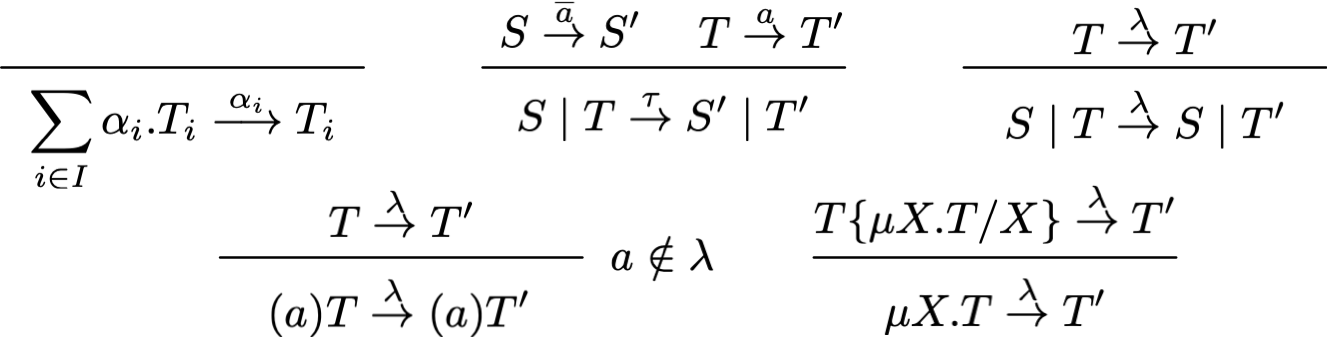
\includegraphics[width=10cm]{../figures/ccs.png}
    \caption[]{\textbf{CCS迁移语义}}
     \label{fig_ccs}
 \end{figure}
   \section{随机进程模型}

   FU Y提供了一个模型无关的方法Uniform Approach(A Uniform Approach to Random Process Model)\cite{Fu_UniformApproach},
   将进程模型扩展为随机进程模型。
   Uniform Approach区分了非确定性行为和概率性行为,
   在CCS的基础上建立了RCCS(Randomized CCS)的语法、迁移语义并研究了RCCS的代数特性,如互模拟关系。

   RCCS在CCS的基础上增加了概率选择操作子$\bigoplus_{i\in I}p_i\tau.T_i$,
   其中$0<p_i<1 \wedge \sum_{i\in I}p_i = 1$。
   例如,$S=\frac{1}{3}\tau.T_1+\frac{2}{3}\tau.T_2$意味着$S$经过静态迁移(内部动作)变迁为$T_1$状态的概率为$\frac{1}{3}$,
   变迁为$T_2$状态的概率为$\frac{2}{3}$。
  对应随机选择操作子的迁移语义如图~\ref{fig_rccs}。
   \begin{figure}[!htbp]
    \small
    \centering
    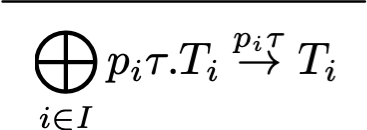
\includegraphics[width=2.5cm]{../figures/rccs.png}
    \caption[]{随机选择操作子的迁移语义}
     \label{fig_rccs}
 \end{figure}

   由于Uniform Approach具有模型无关性,我们可以用它来扩展其他的进程模型,
   进而使非概率模型概率化。

\section{研究目的}
本文希望使用Uniform Approach的通用方法,
概率化扩展经典并发模型——并发传值进程模型,得到随机传值进程模型。
我们可以通过对传值进程模型的扩展,
一方面进一步佐证Uniform Approach的模型无关性;
一方面随机传值进程模型可以应用于具有传值特点的并发系统的建模和分析,
如通信过程、安全协议、生物系统等。
我们希望随机传值进程模型的语法、迁移语义
可以用于为具有传值特点现实问题建模通信、同步等机制,
为这类问题的模型设计与软件开发提供方法,
并可以应用随机传值进程模型的代数特性如互模拟关系、等价关系等
分析模型的死锁、活性、可观察、发散等并发特性。

\section{论文结构}
本文分为四个章节。第\ref{ch:intro}章为绪论,引入了进程演算的概念,
介绍了通信并发演算CCS,引入了一种对进程模型进行概率化扩展的通用方法Uniform Approach。
第\ref{ch:rvpc}章我们使用Uniform Approach中的方法对传值进程模型进行概率化扩展得到随机传值进程模型。
第\ref{ch:gossip}章我们使用随机传值进程模型对基于云计算协议Gossip-Style Membership协议的通信过程建模。
第\ref{ch:conclusion}章为总结以及未来的工作方向。
